La première des alertes que nous proposons de traiter est l'alerte
dite du \emph{Grand Veymont,} issue de l'enregistrement d'un appel au
secours effectué par un accompagnateur en montagne, au sujet d'un de
ses clients.
%
Cette alerte est la plus simple est la plus courte de celles que nous
traiterons ici.

\subsection{Présentation de l'alerte}
\label{subsec:9-2-1}

L'alerte du \emph{Grand Veymont} est l'extrait, d'une durée de 1
minute 06, d'un appel effectué par un accompagnateur en montagne au
sujet d'un de ses clients \autoref{anx:retrans-gv-verb}.


Cette alerte est la plus courte de celles que nous présenterons ici,
elle est composée de 12 extraits, pour un total de 16 expressions.



Pas d'objets multiples

les indications données par le requérant sont assez précises et
détaillées, il est donc possible de définir une \emph{zone initiale de
  recherche} de petite taille. Nous avons défini une \ac{zir} de
\SI{25}{\kilo\meter\squared} (\autoref{fig:zir_grand_veyont}).

\begin{figure}
  \centering
  \begin{tikzpicture}
  \tikzset{et/.style={above,font=\footnotesize\vphantom{Ag}}}
  %
  \node[inner sep=0pt, anchor=south west] (image) at (0,0){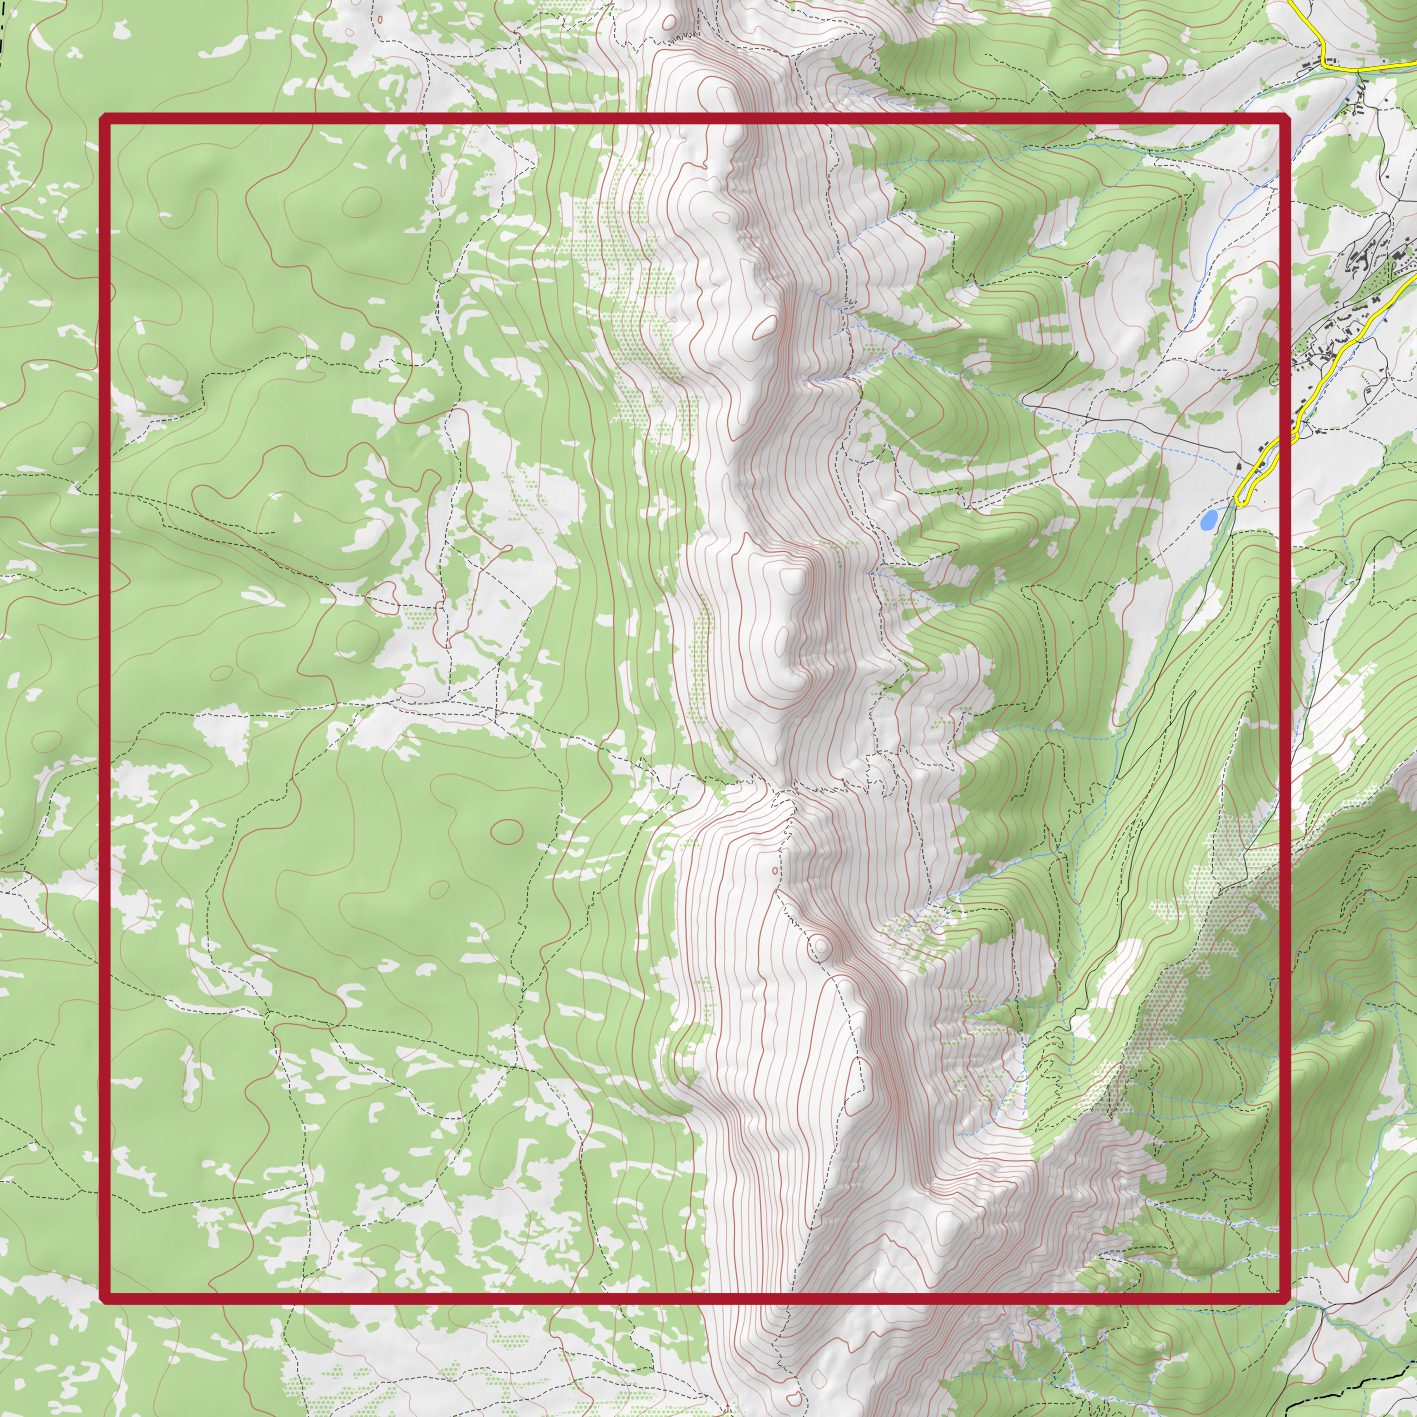
\includegraphics{./figures/ZIR_grand_veymont.png}};
  %
  \begin{scope}
    \node (P2) at ([yshift=-.5cm]image.south east) {};
    \node (P1) at ([yshift=-.5cm]image.south west) {};
    %
    \foreach \x [evaluate=\xshift using \x/10, evaluate=\rad using (\x * .0004) + .01] in {0,...,100}
    {
      \draw[fill=black,draw=none, below] ([xshift=\xshift cm, yshift=-.5cm]P1) circle [radius=\rad cm];
    }
    %
    \path(P1 |- 0cm,-1cm) --++ (10,0)
    node[et,pos=0] {0}
    node[et,pos=.1] {0,1}
    node[et,pos=.2] {0,2}
    node[et,pos=.3] {0,3}
    node[et,pos=.4] {0,4}
    node[et,pos=.65] {0,65}
    node[et,pos=1] {1};
    % Échelle
    \draw[-] (P2 |- -1cm,-1cm) --++ (-1,0) node[et,pos=.5] {\SI{500}{\meter}};
    % Légende détaillée
    \path (P1) -- (P2) node[pos=.5, yshift=-1cm] {\tiny Pour la légende détaillée du fond topographique voir \autoref{anx:topo_leg}. Sources: BD TOPO 2018, BD ALTI 2018.}; 
  \end{scope}
\end{tikzpicture}
  \caption{Zone initiale de recherche pour l'alerte \enquote{Grand Veymont}}
  \label{fig:zir_grand_veyont}
\end{figure}


\subsubsection{Identification des indices de localisation}
\label{subsec:9-2-1-1}


Pour construire la zone de localisation probable de cette alerte il
est nécessaire d'en identifier les différents indices de localisation
et de sélectionner la relation de localisation la plus adaptée à leur
modélisation. Comme nous le signalions précédemment, ce travail est
prévu pour être réalisé parle secouriste durant l'alerte et non à
posteriori.Pour identifier les relations de localisation utilisables
pour modéliser les différents indices de localisation données par le
requérant nous allons nous appuyer sur le verbatim de la discussion
téléphonique entre le requérant et le secouriste, ainsi que son
découpage en \emph{expressions,} réalisé durant la phase de
retranscription (\autoref{chap:05}). Le verbatim complet de l'alerte
est donné dans la \autoref{anx:retrans-gv-verb}. On pourra remarquer
que certains détails présents dans la retranscription en annexe (qui
fait office de référence) ne figurent pas ici, notamment les
hésitations ou les bafouillements. Les extraits que nous faisons
figurer ici ne correspondent donc pas exactement à la discussion
réelle, même si nous avons tout fait pour ne pas altérer le sens des
propos tenus.

Le requérant commence par décrire sa position en donnant plusieurs
éléments de contexte :
%
\begin{dialogue*}
  % 
  \Req \lnex{1}{gv:1} J'ai eu du mal à descendre entre le sommet du
  \emph{Grand Veymont} et là où je suis. \lnex{2}{gv:2} La descente
  était très très lente.
\end{dialogue*}
%
Ces deux premiers extraits ne peuvent pas être retranscrits à l'aide
d'une des relations spatiales que nous avons définies. En effet,
l'extrait \ref{gv:1} ne décrit pas la position actuelle du requérant,
mais la \emph{configuration} du chemin qu'il a emprunté pour atteindre
cette position. On pourrait supposer que la relation de localisation
\onto[orl]{Sous\-Jalon\-Sur\-Iti\-ne\-rai\-re} est pertinente dans ce
cas. Cependant l'utilisation de cette relation de localisation
nécessite que le site soit un jalon de l’itinéraire actuel du
requérant, or, rien ici ne permet d'affirmer que c'est toujours le
cas. De plus, nous ne savons pas si le requérant est toujours situé
sur un sentier, bien que cette hypothèse paraisse légitime, elle ne
doit pas être systématisée. Ce premier extrait ne nous permet donc pas
d'identifier un indice de localisation.

On peut cependant extrapoler certaines informations de ces deux
extraits. Par exemple, on peut légitimement considérer que le
requérant n'est plus sur le sommet du \emph{Grand Veymont,} ce que
l'on peut alors traduire par la relation de localisation
\onto[orl]{Hors\-De\-Planimétrique}, indiquant que la cible est à
l'extérieur du site. Dans le contexte de l'alerte, le site est le
sommet du \emph{Grand Veymont,} sont étendue est donc particulièrement
réduite. Par conséquent la \ac{zlc} de cet indice sera de grande
taille, ce qui rend cet indice de localisation peu discriminant.

L'extrait \ref{gv:2} ne donne quant à lui pas d'informations sur la
position actuelle du requérant. Il donne cependant une idée de la
vitesse de déplacement du requérant durant la descente et permet de
conclure que la distance parcourue est vraisemblablement inférieure à
celle qu'aurai parcouru le même groupe dans des conditions
normales. Néanmoins, comme notre travail ne porte pas sur l'analyse de
déplacements, nous ne pouvons exploiter cette information.

Les premiers indices donnant une information réellement discriminante
sont ceux que l'on peut construire à partir des extraits \ref{gv:3} et
\ref{gv:4}, plus riches :
%
\begin{dialogue*}
  % 
  \Sec \lnex{3}{gv:3} Vous êtes entre \emph{Grand Veymont} et
  \emph{Pas de la Ville} ?

  \Req \lnex{4}{gv:4} Je suis entre le \emph{Grand Veymont,}
  \lnex{5}{gv:5} sous le \emph{Grand Veymont} et \emph{Pas de la
    Ville,} tout à fait, \lnex{6}{gv:6} coté sud.
\end{dialogue*}
% 
Les extraits \ref{gv:3} et \ref{gv:4} indiquent que le requérant se
situe entre le \emph{Grand Veymont} et le \emph{Pas de la Ville,} ce
que l'on peut modéliser avec la \emph{relation de localisation}
\onto[orl]{Entre\-X\-et\-Y}. Bien que ce ne soit pas explicitement
mentionné dans l'extrait, on comprend à l'aide du contexte et de
l'extrait \ref{gv:1} que le requérant se réfère ici au \emph{sommet}
du \emph{Grand Veymont} et non à la montagne dans son ensemble. Le
même problème se pose pour l'extrait \ref{gv:5}, où le requérant
indique que sa position est située en dessous du \emph{Grand Veymont,}
sans expliciter qu'il s'agit du sommet. Une nouvelle fois le contexte
et l'extrait \ref{gv:1} nous permettent de conclure que le requérant
se réfère ici au sommet du \emph{Grand Veymont.} On peut donc ajouter
un second indice de localisation, utilisant une relation de
localisation retranscrivant la relation de verticalité existant entre
le requérant et le site, comme \onto[orl]{Sous\-Altitude}. Nous avons
certes défini plusieurs relations de localisation dérivées de cette
dernière, comme \onto[orl]{Sous\-Proche\-De} et permettant une
spatialisation plus fine, mais aucune d'entre elles ne nous semble
adaptée à la situation. La relation de localisation
\onto[orl]{Sous\-Proche\-De}, par exemple, contraint l'éloignement au
site. Or, rien dans les extraits de cette alerte ne permet d'affirmer
que le requérant est proche du site, au contraire, des extraits comme
le \ref{gv:1} ou le \ref{gv:5} laissent supposer que le requérant
s'est déjà considérablement éloigné du sommet du \emph{Grand Veymont.}
De la même manière, la relation de localisation
\onto[orl]{Sous\-A\-L\-Aplomb\-De} ne nous semble pas adaptée pour
représenter la sémantique de cet extrait. En effet, cette relation de
localisation contraint la \ac{zlc} suivant l'axe de plus grande pente
(\autoref{anx:orl_dic}). Cette contrainte nous semble ici trop
restrictive, aucun élément de l'alerte ne permettant d'affirmer qu'une
telle relation existe ici. Quant à la relation de localisation
\onto[orl]{Sous\-Jalon\-Sur\-Itineraire}, cette dernière contraint la
relation de localisation \onto[orl]{Sous\-Altitude}, par la position
des itinéraires, or, comme nous l'avons déjà signalé il n'est pas
nécessairement pertinent de considérer que c'est le cas ici.

Dans l'extrait \ref{gv:6}, le requérant complète cette information en
précisant sa position par une relation de localisation
cardinale. Cette description est cependant interprétable, car le
requérant n'en précise pas le cadre de référence, ce qui est relevé
par le secouriste :
%
\begin{dialogue*}
  %
  \Sec \lnex{7}{gv:7} Côté Sud du \emph{Pas de la Ville} ?
%
  \Req \lnex{8}{gv:8} Non, côté Nord.
\end{dialogue*}
%
Dans ce contexte il est difficile de savoir si les extraits \ref{gv:6}
et \ref{gv:8} se contredisent et que le requérant est revenu sur sa
précédente déclaration, ou, si l'extrait \ref{gv:6} ce référait
implicitement au sommet du \emph{Grand Veymont} et non au \emph{Pas de
  la Ville.} Si l'on observe le cadre géographique de l'alerte
(\autoref{fig:zir_grand_veyont}) on peut remarquer que seules trois
configurations sont possibles :
%
\begin{enumerate*}[label=(\arabic*)]
\item le requérant est au nord du \emph{Grand Veymont} et du \emph{Pas
    de la Ville},
\item le requérant est au nord du \emph{Grand Veymont} et au sud du
  pas de la Ville, et
\item le requérant est au sud du \emph{Pas de la Ville} et du
  \emph{Grand Veymont.}
\end{enumerate*}
%
Parmi ces trois configurations, seule la seconde est compatible avec
l'extrait \ref{gv:4}, indiquant que le requérant est \emph{entre} le
sommet du \emph{Grand Veymont} et le \emph{Pas de la Ville.} Les deux
autres possibilités impliquant que le requérant ait dépassé l'un de
deux sites, ce qui invalidait l'affirmation de l'extrait
\ref{gv:4}. C'est, cependant, ce que tendent à faire les extraits
suivants :
%
\begin{dialogue*}
  % 
  \Sec \lnex{9}{gv:9} Vous êtes au-delà du \emph{Pas de la Ville ?}
  \lnex{10}{gv:10} Entre \emph{Pas de la ville} et \emph{Pierre
    Blanche ?}
  % 
  \Req \lnex{11}{gv:11} Oui, je suis au-delà du \emph{Pas de la
    Ville.}
\end{dialogue*}
%
Si l'on se réfère une nouvelle fois à la
\autoref{fig:zir_grand_veyont} on peut en effet constater qu'il est
difficile d'identifier une zone étant ---~même partiellement~--- à la
fois entre le sommet du \emph{Grand Veymont} et le \emph{Pas de la
  Ville} et entre le \emph{Pas de la Ville} et le sommet de
\emph{Pierre Blanche,} ces trois géotypes étant quasiment alignés. De
la même manière, on ne peut être \emph{entre} le sommet du \emph{Grand
  Veymont} et le \emph{Pas de la Ville} et en même temps,
\emph{au-delà} du \emph{Pas de la Ville} en étant parti du sommet du
\emph{Grand Veymont.} Ces différents extraits se contredisent.

Deux choix s'offrent alors à nous. On peut considérer que les extraits
\ref{gv:9} à \ref{gv:11} sont plus dignes de confiance que l'extrait
\ref{gv:4}, ou l'inverse. Le déroulé de l'alerte nous laisse supposer
que la première solution, attribuant une meilleure confiance aux
extraits \ref{gv:9} à \ref{gv:11} est la meilleure, le secouriste
ayant cherché à invalider l'extrait \ref{gv:6}, lors de l'extrait
\ref{gv:7} et préciser les réponses du requérant lors des extraits
\ref{gv:9} et \ref{gv:10}. L'incompatibilité entre ces indices étant
manifeste et la fausseté de l'extrait \ref{gv:4} étant certaine, on
peut dès lors rejeter l'indice de localisation défini à partir de
l'extrait \ref{gv:4} directement et non en diminuer légèrement la
confiance, comme on serait tenté de le faire. Le rejet de cet indice
de localisation invalide notre précédente interprétation des extraits
\ref{gv:6} et \ref{gv:8}. Les extraits \ref{gv:9} à \ref{gv:11}
s'opposent en effet à ce que la position du requérant soit située au
sud du \emph{Pas de la Ville,} ainsi, la seule configuration cohérente
avec le reste des extraits est celle où le requérant est situé au nord
du \emph{Pas de la Ville} et du \emph{Grand Veymont}.

On peut donc envisager de modéliser l'extrait \ref{gv:8} avec la
relation de localisation de localisation \onto[orl]{Au\-Nord\-De}, ou
une de ses relations filles, \onto[orl]{Dans\-La\-Partie\-Nord\-De} et
\onto[orl]{Au\-Nord\-De\-Externe}. La relation de localisation
\onto[orl]{Dans\-La\-Partie\-Nord\-De} ajoute une contrainte à la
relation de localisation \onto[orl]{Au\-Nord\-De}, la présence de la
cible au sein du site. À l'inverse, la relation de localisation
\onto[orl]{Au\-Nord\-De\-Externe} impose que la cible soit en dehors
du site. Dans le cas de cette alerte on peut rapidement rejeter
l'utilisation de la relation \onto[orl]{Dans\-La\-Partie\-Nord\-De},
le Pas de la Ville n'étant pas un site suffisamment vaste pour qu'il
soit nécessaire de préciser sa position en son sein. L'extrait
\ref{gv:8} ne suffit pas à lui seul pour trancher entre les relations
de localisation \onto[orl]{Au\-Nord\-De} et
\onto[orl]{Au\-Nord\-De\-Externe}. Cependant, les extraits suivants
(\ref{gv:9} et \ref{gv:11}) indiquent que le requérant est
\emph{au-delà} du \emph{Pas de la Ville,} ce qui implique qu'il ait
dépassé cet objet de référence, ce qui fait de la relation de
localisation \onto[orl]{Au\-Nord\-De\-Externe}, la plus adaptée à la
modélisation de l'extrait \ref{gv:8}.

Pour modéliser les extraits \ref{gv:9} et \ref{gv:10}.

Les questions posées par le secouriste dans les extraits \ref{gv:9} et
\ref{gv:10}
%
On ne peut, en effet, pas considérer que les prépositions
\enquote{entre} (\ref{gv:10}) et \enquote{au-delà} (\ref{gv:9}) sont
utilisées comme synonymes.
%
Pourtant, en confirmant qu'il est \enquote{au-delà} du \emph{Pas de la
  Ville} (\ref{gv:11}) le requérant contredit sa précédente
affirmation (\ref{gv:4}), comme quoi il serait situé entre le
\emph{Pas de la Ville} et le \emph{Grand Veymont.}

Viennent ensuite les extraits \ref{gv:12} et \ref{gv:13} :
%
\begin{dialogue*}
  \Req \lnex{12}{gv:12} Sur une zone à peu près plate et
  caillouteuse. \lnex{13}{gv:13} Sur une petite prairie.
\end{dialogue*}
%
L'interprétation de ces deux extrais ne présente pas de difficulté
particulière. Tous deux décrivent en effet la nature du terrain pour
la position actuelle du requérant. Dit autrement, ces deux extraits
indiquent que le requérant est \emph{dans} \enquote{une à peu près
  plate et caillouteuse} (\ref{gv:12}), mais également \emph{dans}
\enquote{une petite prairie} (\ref{gv:13}). La relation de
localisation destinée à modéliser l'inclusion de la cible dans le site
est \onto[orl]{Dans\-Planimetrique}. Comme nous le verrons lors de la
spatialisation des indices, dans ce cas particulier c'est la
délimitation des objets de référence à utiliser qui peut présenter
certaines difficultés.

Les deux derniers extraits de l'alerte décrivent l'éloignement de la
position du requérant au \emph{Pas de la ville :}
%
\begin{dialogue*}
  \Sec \lnex{14}{gv:14} Vous êtes à combien du Pas de la ville ?
  % 
  \Req \lnex{15}{gv:15} À 800 mètres, je crois, à vol d'oiseau.
\end{dialogue*}
%
Comme précédemment, l'interprétation de ces deux extraits ne pose pas
de problèmes particuliers. Le requérant précise clairement la nature
de la distance qu'il décrit, il s'agit d'une distance à vol d'oiseau,
visuellement approximée. Une relation de localisation
\onto[orl]{Distance\-Quanti\-ta\-ti\-ve\-Plani\-metrique} est dédiée à
la modélisation de ce type d'indices de localisation. L'extrait
\ref{gv:15} met cependant en évidence le fait que le requérant est
particulièrement hésitant dans sa réponse
(\autoref{anx:retrans-gv-verb}), sa certitude en la validité de cette
description semble donc assez faible. Nous ne pouvons qu'imaginer la
confiance qu'un secouriste attribuerait à cet indice de localisation,
mais il nous semble très probable qu'elle serait plus faible que celle
des autres indices. C'est pourquoi nous proposons d'attribuer une
confiance moyenne à cet indice de localisation.


Au terme de l'analyse de la retranscription de l'alerte on peut
construire un ensemble d'indices (\autoref{eq:ens_ind_loc}), composé
de 9 indices de localisation différents et non contradictoires :
%
\begin{enumerate}
\item Le requérant est \onto[orl]{Hors\-De\-Planimetrique} du sommet
  du \emph{Grand Veymont}
  % 
\item Le requérant est \onto[orl]{Sous\-Altitude} du sommet du
  \emph{Grand Veymont}
  % 
\item Le requérant est \onto[orl]{Au\-Nord\-De\-Externe} du \emph{Pas
    de la Ville}
  % 
\item Le requérant est \onto[orl]{XX} du \emph{Pas de la Ville,} par
  rapport au sommet du \emph{Grand Veymont}
  % 
\item Le requérant est \onto[orl]{EntreXetY} le \emph{Pas de la ville}
  est \emph{Pierre Blanche}
  % 
\item Le requérant est \onto[orl]{Dans\-Planimétrique} une zone à peu
  près plate
  % 
\item Le requérant est \onto[orl]{Dans\-Planimétrique} une zone
  caillouteuse
  % 
\item Le requérant est \onto[orl]{Dans\-Planimétrique} une petite
  prairie
  % 
\item Le requérant est \onto[orl]{Distance\-Quantitative} de
  \SI{800}{\meter}, avec une certitude moyenne, du \emph{Pas de la
    Ville}
\end{enumerate}

Chacun de ces indices de localisation peut à présent être traité,
conformément à la méthode que nous avons présenté dans les chapitres
\ref{chap:06} à \ref{chap:08}.

\subsection{Modélisation de l'alerte}
\label{subsec:9-2-2}

La première étape de notre méthode (\autoref{fig:methodo_1}) consiste
à décomposer l'ensemble des indices de localisation en plusieurs
indices indépendants, traités séparément les uns des autres. Comme
nous l'expliquions dans le chapitre dédié à la phase de décomposition
(\autoref{chap:05}), cette première étape est triviale, les indices de
localisation étant décomposés dès leur saisie. Dans le cas de l'alerte
\emph{Grand Veymont} on a donc 9 indices de localisation, dans
l'ensemble assez simples à spatialiser, comme nous allons le voir.

Pour des raisons de lisibilité nous présenterons l'ensemble des
opérations permettant de passer des indices de localisation identifiés
précédemment à leur \ac{zlc}, en regroupant dans une même partie la
décomposition des objets de référence et de relations de localisation,
la spatialisation, la fusion de relations de localisation atomiques et
des objets de référence indéfinis. Seule la fusion des \ac{zlc} des
différents indices en vue de la construction de la \ac{zlp} sera
séparée du reste.

\subsubsection{XXX}

Si l'on converse l'ordre des extraits, le premier des indices de
localisation est \enquote{le requérant est
  \onto[orl]{Hors\-De\-Planimetrique} du sommet du \emph{Grand
    Veymont}}. Pour construire la \ac{zlc} correspondant a cet indice
de localisation il est nécessaire de poursuivre la phase de
décomposition (\autoref{fig:methodo_1}). Ici, l'objet de référence de
l'indice de localisation est nommé, il s'agit du sommet du \emph{Pas
  de la Ville.} Par conséquent, il n'est pas nécessaire de décomposer
selon les objets de référence indéfinis. De plus, comme nous
l'expliquions dans le \autoref{chap:07}, la relation de localisation
\onto[orl]{Hors\-De\-Planimetrique} est, comme la relation
\onto[orl]{Dans\-Planimetrique} à laquelle elle s'oppose
(\autoref{fig:ex_parties_statialisation_dansplani}), une relation de
localisation atomique. Il n'est donc pas nécessaire de décomposer la
relation de localisation. Ainsi, ce premier indice de localisation est
directement spatialisable.

Étant donné que la relation de localisation
\onto[orla]{Hors\-De\-Pla\-ni\-mé\-tri\-que} s'oppose à la relation
\onto[orla]{Dans\-Planimetrique}, déjà présentée
(\autoref{fig:ex_parties_statialisation_dansplani}), on peut
spatialiser les deux concepts de manière assez semblable. Ces deux
relations sont, en effet, spatialisées avec le même rasteriser et la
même métrique, seul le fuzzyficateur les distingue
(\autoref{fig:ex_parties_statialisation_horsdeplani}). Nous avons déjà
détaillé les raisons du choix de ce rasteriser et de cette métrique
pour la relation \onto[orla]{Dans\-Planimetrique} dans le
\autoref{chap:07}. L'utilisation du fuzzyficateur \onto[otla]{Sup\-0}
permet quand à elle d'attributer un degré d'appartenance non nul aux
positions pour lesquelles la distance à l'objet de référence est
supérieure à zéro, c'est-à-dire aux positions situées à l'extérieur de
l'objet de référence.

\begin{figure}
  \centering
  \begin{tikzpicture} 
  \node[anchor=east] (x1) at (-3.5,0) {\onto[orla]{Hors\-De\-Planimétrique}};

  \node[anchor=west] (y1) at (3.5,.8) {\onto[orla]{Geometrie}};
  \node[anchor=west] (y2) at (3.5,0) {\onto[orla]{Distance}};
  \node[anchor=west] (y3) at (3.5,-0.8) {\onto[orla]{Sup\-Val\-0}};
  
  \fill[RdBu-9-9] (x1.east) circle (2pt);
  
  \fill[RdBu-9-1] (y1.west) circle (2pt);
  \fill[RdBu-9-1] (y2.west) circle (2pt);
  \fill[RdBu-9-1] (y3.west) circle (2pt);

  \draw[->, shorten >=5pt, shorten <=5pt] (x1.east) |- (y1.west)
  node[pos=0.75, sloped, anchor=center, fill=white] {\tiny\emph{A pour rasteriser}};
  
  \draw[->, shorten >=5pt, shorten <=5pt] (x1.east) -- (y2.west)
  node[pos=0.5, sloped, anchor=center, fill=white] {\tiny\emph{A pour métrique}};

    \draw[->, shorten >=5pt, shorten <=5pt] (x1.east) |- (y3.west)
  node[pos=0.75, sloped, anchor=center, fill=white] {\tiny\emph{A pour fuzzyficateur}};
\end{tikzpicture}
  \caption{\emph{Rasteriser,} \emph{métrique} et \emph{fuzzyficateur}
    utilisés pour la \emph{spatialisation} de la \emph{relation de
      localisation atomique}
    \protect\onto[orla]{Hors\-De\-Pla\-ni\-mé\-tri\-que}.}
  \label{fig:ex_parties_statialisation_horsdeplani}
\end{figure}

Dans le cas particulier de cet indice de localisation, l'objet de
référence est un point


On peut alors calculer la métrique à partir de cette rasterisation. La
\autoref{fig:Distance_GrandVeymont} représente le résultat du calcul
de la métrique \onto[orla]{Distance} pour toutes les positions de la
\ac{zir} \footnote{Pour des raisons de lisibilité de la représentation
  graphique, la résolution de la représentation a été réduite à 50
  mètres, pour toutes les figures représentant les résultats de la
  modélisation de l'alerte \emph{Grand Veymont.} Le calcul a cependant
  été réalisé avec une résolution de 5 mètres.} à partir du sommet du
\emph{Grand Veymont.}

\begin{figure}
  \centering
  \input{./figures/Distance_GrandVeymont.tex}
  \caption{Distance euclidienne au sommet du \enquote{Grand Veymont}}
  \label{fig:Distance_GrandVeymont}
\end{figure}


\begin{figure}
  \centering
  \begin{tikzpicture}[scale=.7]
  \def\decalageX{-.2}
  \def\decalageY{-.2}
  % Courbe
  \begin{scope}[transparency group]
    % fond
    \begin{scope}
      \path[ffa]  (3,0) -- (6, 2)  -- (8,2) -- (8,0) -- cycle;
      \path[ffa_fade]  (8,2) -- (9, 2)  -- (9,0) -- (8,0) -- cycle;
    \end{scope}
    % bords
    \begin{scope}
      \path[ffc_fade_m] (0,0) -- (2,0) ;
      \path[ffc] (2,0) -- (3,0) -- (6, 2) -++ (3,0) ;
      \path[ffc_fade] (8,2) -- (9,2) ;
    \end{scope}
  \end{scope}
  % Axes X, Y
  \begin{scope}
    % Axe X
    \begin{scope}
      % Axe
      \draw[<->] (0, \decalageX) --++ (9, 0) coordinate (x axis);
      % Graduations
      \foreach \n/\t in {1/{},2/{},3/{},4/{},5/{},6/{0},7/{},8/{}}
      {
        \draw[-] (\n, \decalageX - .05) --++ (0, .1);
        \node[below, font=\footnotesize] at (\n, \decalageX - .05) {\t};
      }
      % label
      \node[below left, yshift=-.1cm, font=\small] at (x axis) {\itshape Métrique};
    \end{scope}
    % Axe Y
    \begin{scope}
      % Axe
      \draw[-] (\decalageY ,0) --++ (0, 2) coordinate (y axis);
      % Graduations
      \foreach \n/\t in {0/{0},2/{1}}
      {
        \draw[-] (\decalageY -.05, \n) --++ (.1, 0);
        \node[left, font=\footnotesize] at (\decalageY -.05, \n) {\t};
      }
      % Label
      \node[above] at (y axis) {$\mu$};
    \end{scope}
  \end{scope}
  \begin{scope}
    % Seuil 1
    \draw[ffc,line width=.5] (3,\decalageY) -- (3,0);
    \draw[fill, RdBu-9-1] (3,\decalageY) circle (2pt);
    \draw[fill, RdBu-9-1] (3,0) circle (2pt);
    % Seuil 2
    \draw[ffc,line width=.5] (6,\decalageY) -- (6,2);
    \draw[fill, RdBu-9-1] (6,\decalageY) circle (2pt);
    \draw[fill, RdBu-9-1] (6,2) circle (2pt);
    \node[above] at (6,2) {\(v\)};

    \draw[|-] (3,-.7cm) --++(2.7,0) node[pos=.5, fill=white, inner
    sep=1pt, font=\small] {$\delta$};
  \end{scope}
\end{tikzpicture}

  \caption{Fonction d'appartenance pour le fuzzyficateur
    \protect\onto[orla]{Sup\-0}, paramétrée.}
  \label{fig:fuzzy_veyont_distanceSommet}
\end{figure}


\begin{figure}
  \centering
  \input{./figures/Distance_GrandVeymont.tex}
  \caption{Zone de localisation compatible pour l'indice de
    localisation 1}
  \label{fig:ZLC_GrandVeymont_1}
\end{figure}

\subsubsection{Sous Altitude Grand Veymont}

Le second indice de localisation défini est :

Comme nous l'avons détaillé dans le \autoref{chap:07}, la relation de
localisation \onto[orl]{Sous\-Altitude} est une relation de
localisation atomique, ayant \onto[orla]{Geometrie} comme rasteriser,
\onto[orla]{Delta\-Nearest\-Val} comme métrique et
\onto[orla]{Inf\-Val\-0} comme fuzzyficateur
(\autoref{fig:ex_parties_statialisation_sousalt}).

L'objet de référence étant le même que pour le précédent indice


La métrique

% \begin{figure}
%   \centering
%   \input{./figures/Distance_GrandVeymont.tex}
%   \caption{Distance euclidienne au sommet du \enquote{Grand Veymont}}
%   \label{fig:Distance_GrandVeymont}
% \end{figure}


La fonction d'appartenance utilisée pour la fuzzyfication de  

% \begin{figure}
%   \centering
%   \begin{tikzpicture}[scale=.7]
  \def\decalageX{-.2}
  \def\decalageY{-.2}
  % Courbe
  \begin{scope}[transparency group]
    % fond
    \begin{scope}
      \path[ffa]  (3,0) -- (6, 2)  -- (8,2) -- (8,0) -- cycle;
      \path[ffa_fade]  (8,2) -- (9, 2)  -- (9,0) -- (8,0) -- cycle;
    \end{scope}
    % bords
    \begin{scope}
      \path[ffc_fade_m] (0,0) -- (2,0) ;
      \path[ffc] (2,0) -- (3,0) -- (6, 2) -++ (3,0) ;
      \path[ffc_fade] (8,2) -- (9,2) ;
    \end{scope}
  \end{scope}
  % Axes X, Y
  \begin{scope}
    % Axe X
    \begin{scope}
      % Axe
      \draw[<->] (0, \decalageX) --++ (9, 0) coordinate (x axis);
      % Graduations
      \foreach \n/\t in {1/{},2/{},3/{},4/{},5/{},6/{0},7/{},8/{}}
      {
        \draw[-] (\n, \decalageX - .05) --++ (0, .1);
        \node[below, font=\footnotesize] at (\n, \decalageX - .05) {\t};
      }
      % label
      \node[below left, yshift=-.1cm, font=\small] at (x axis) {\itshape Métrique};
    \end{scope}
    % Axe Y
    \begin{scope}
      % Axe
      \draw[-] (\decalageY ,0) --++ (0, 2) coordinate (y axis);
      % Graduations
      \foreach \n/\t in {0/{0},2/{1}}
      {
        \draw[-] (\decalageY -.05, \n) --++ (.1, 0);
        \node[left, font=\footnotesize] at (\decalageY -.05, \n) {\t};
      }
      % Label
      \node[above] at (y axis) {$\mu$};
    \end{scope}
  \end{scope}
  \begin{scope}
    % Seuil 1
    \draw[ffc,line width=.5] (3,\decalageY) -- (3,0);
    \draw[fill, RdBu-9-1] (3,\decalageY) circle (2pt);
    \draw[fill, RdBu-9-1] (3,0) circle (2pt);
    % Seuil 2
    \draw[ffc,line width=.5] (6,\decalageY) -- (6,2);
    \draw[fill, RdBu-9-1] (6,\decalageY) circle (2pt);
    \draw[fill, RdBu-9-1] (6,2) circle (2pt);
    \node[above] at (6,2) {\(v\)};

    \draw[|-] (3,-.7cm) --++(2.7,0) node[pos=.5, fill=white, inner
    sep=1pt, font=\small] {$\delta$};
  \end{scope}
\end{tikzpicture}

%   \caption{Fonction d'appartenance pour le fuzzyficateur
%     \protect\onto[orla]{Sup\-0}, paramétrée.}
%   \label{fig:fuzzy_veyont_distanceSommet}
% \end{figure}

On obtient alors la \ac{zlc} de ce second indice de localisation.

% \begin{figure}
%   \centering
%   \input{./figures/Distance_GrandVeymont.tex}
%   \caption{Zone de localisation compatible pour l'indice de
%     localisation 1}
%   \label{fig:ZLC_GrandVeymont_2}
% \end{figure}

\subsubsection{Au nord du Pas de la Ville}

La relation de localisation \onto[orl]{Au\-Nord\-De\-Externe},
utilisée pour modéliser le troisième indice de localisation est la
première des relations de localisation non atomiques de cette alerte.
%
Cette relation se décompose en deux relation de localisation
atomiques, \onto[orla]{Au\-Nord\-De} et
\onto[orla]{Hors\-De\-Planimétrique}. La relation de localisation
atomique \onto[orla]{Au\-Nord\-De} \footnote{Que la relation de
  localisation \protect\onto[orla]{Au\-Nord\-De\-Externe} partage avec
  sa relation sœur \protect\onto[orla]{Dans\-La\-Partie\-Nord\-De}.}


\begin{figure}
  \centering
  \begin{tikzpicture}
  \tikzset{et/.style={above,font=\footnotesize\vphantom{Ag}}}
  % 
  \node[inner sep=0pt, anchor=south west] (image) at (0,0){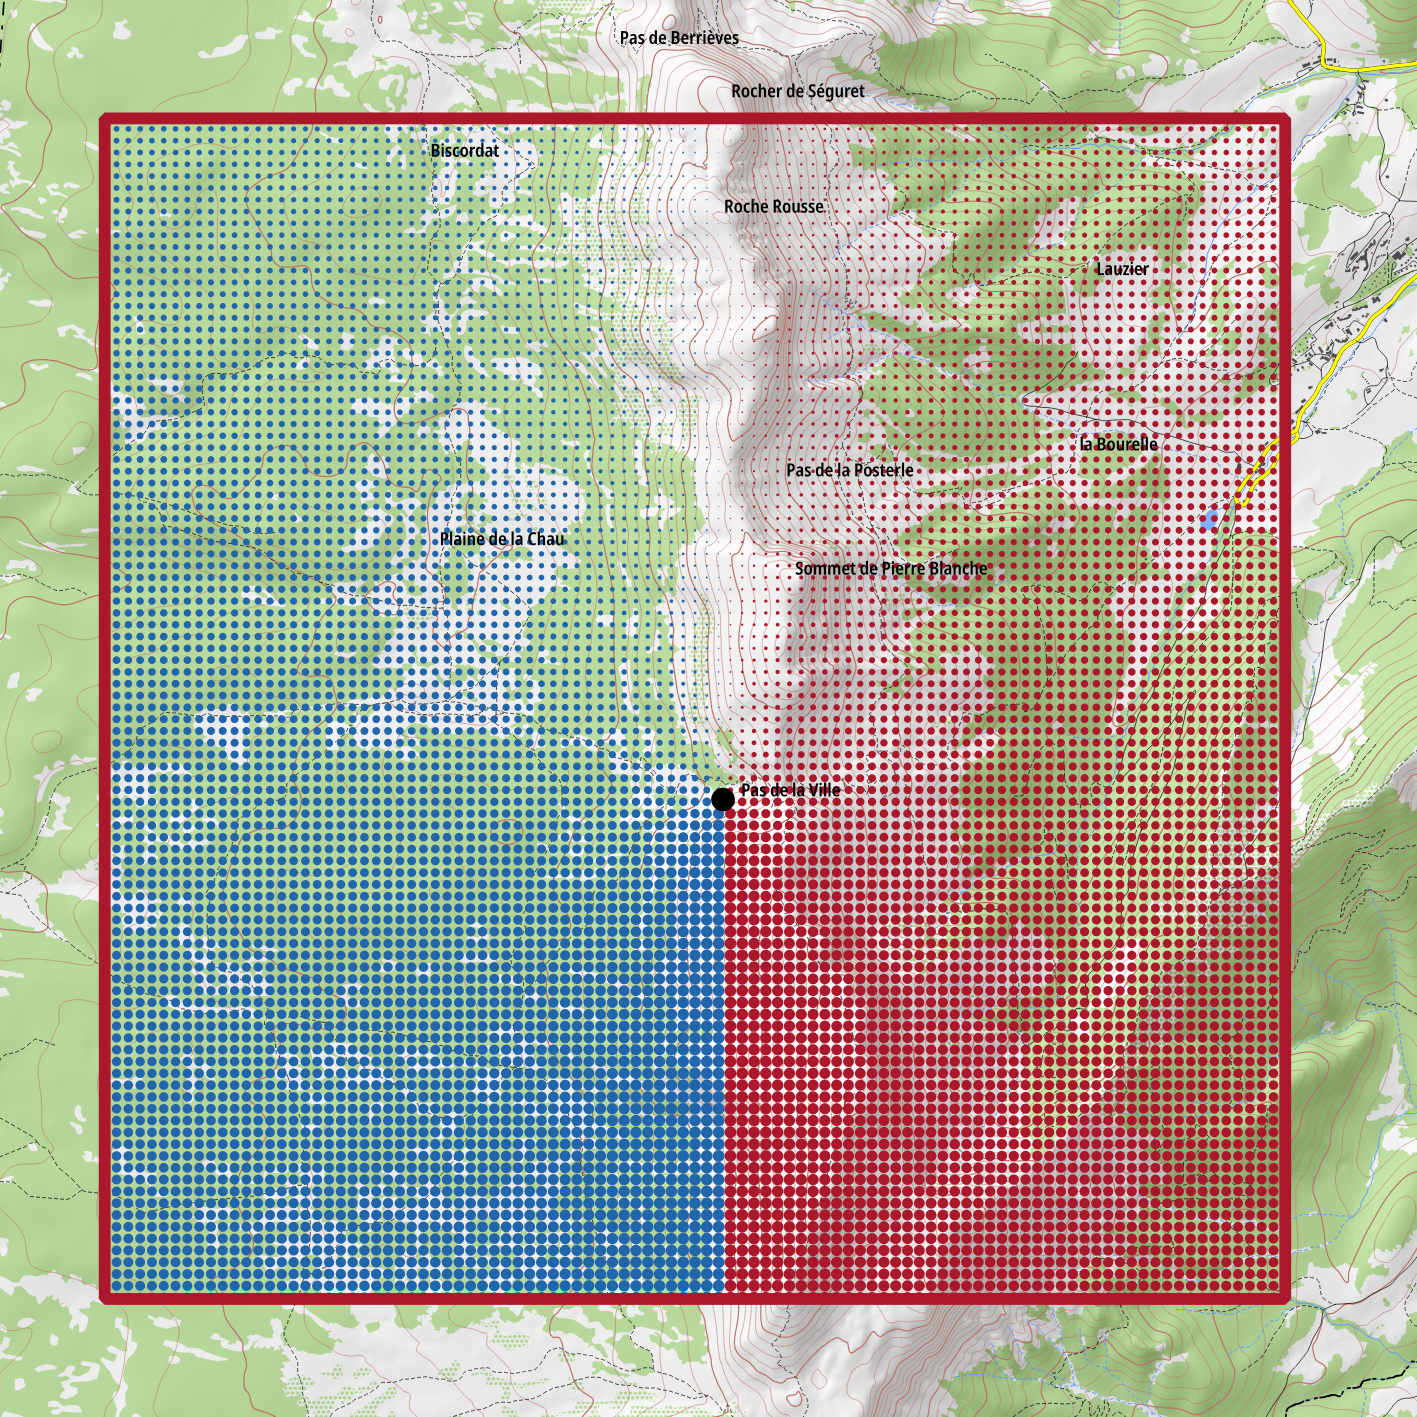
\includegraphics{./figures/EcartNord_PasVille.png}};
  % 
  \begin{scope}
    \node (P2) at ([yshift=-.5cm]image.south east) {};
    \node (P1) at ([yshift=-.5cm]image.south west) {};
    % 
    \node (rect) [anchor=north west, minimum width=1cm,minimum
    height=.25cm] at ([yshift=-.25cm]P1) {}; \path[draw=RdBu-9-1, line
    width=1mm](rect.west) --([xshift=-1ex]rect.south) -- ([xshift=1ex]rect.north)
    -- (rect.east);
    % 
    \node[anchor=west, font=\tiny\vphantom{Ag}, text width = 4cm] at
    ([xshift=1ex]rect.east) {Limite de la \ac{zir}};
    %
    \node[anchor=west, font=\footnotesize\vphantom{Ag}, text width=8cm] at
    (P1 |- 0cm,-1.85cm) {Écart angulaire à la demi-droite passant par
      le \emph{Pas de la Ville} et orientée au nord :};
    %
    \begin{scope}
      \foreach \x [evaluate=\xshift using 1+\x/10, evaluate=\rad using (\x * -.0008) + .05] in {0,...,50}
      {
        \draw[fill=RdBu-9-1,draw=none, below] ([xshift=\xshift cm, yshift=-2.5cm]P1) circle [radius=\rad cm];
      }
      \foreach \x [evaluate=\xshift using 6+\x/10, evaluate=\rad using (\x * .0008) + .01] in {0,...,50}
      {
        \draw[fill=RdBu-9-9,draw=none, below] ([xshift=\xshift cm, yshift=-2.5cm]P1) circle [radius=\rad cm];
      }
      % 
      \path(1,-3) --++ (10,0)
      node[et,pos=0] {\SI{180}{\degre}}
      node[et,pos=.5] {\SI{0}{\degre}}
      node[et,pos=1] {\SI{-180}{\degre}};
    \end{scope}

    % Échelle
    \draw[-] (P2 |- -1cm,-1cm) --++ (-1,0) node[et,pos=.5] {\SI{500}{\meter}};
    % Légende détaillée
    \path (P1) -- (P2) node[pos=.5, yshift=-3cm] {\tiny Pour la légende détaillée du fond topographique voir \autoref{anx:topo_leg}. Sources: BD TOPO 2018, BD ALTI 2018.}; 
  \end{scope}
\end{tikzpicture}
  \caption{Métrique \protect\onto[orla]{Ecart\-Angulaire}, calculée
    pour la spatialisation de la relation de localisation
    \protect\onto[orl]{AuNordDe}. La résolution du raster a
    été réduite de 5 à 50 mètres pour la représentation.}
  \label{fig:veyont_EcartNord}
\end{figure}


% \begin{figure}
%   \centering
%   \begin{tikzpicture}[scale=.7]
  \def\decalageX{-.2}
  \def\decalageY{-.2}
  % Courbe
  \begin{scope}[transparency group]
    % fond
    \begin{scope}
      \path[ffa]  (3,0) -- (4.5, 2) -- (6,0) -- cycle;
    \end{scope}
    % bords
    \begin{scope}
      \path[ffc] (1,.8) -- (3.6,.8) -- (4.5, 2) -- (5.4,.8) -- (8,.8) ;
      \path[ffc_fade_m] (0,.8) -- (1,.8) ;
      \path[ffc_fade] (8,.8) -- (9,.8) ;
    \end{scope}
  \end{scope}
  % Axes X, Y
  \begin{scope}
    % Axe X
    \begin{scope}
      % Axe
      \draw[<->] (0, \decalageX) --++ (9, 0) coordinate (x axis);
      % Graduations
      \foreach \n/\t in {0.5/{},1.5/{},2.5/{400},3.5/{},4.5/{800},5.5/{},6.5/{1200},7.5/{},8.5/{}}
      {
        \draw[-] (\n, \decalageX - .05) --++ (0, .1);
        \node[below, font=\footnotesize] at (\n, \decalageX - .05) {\t};
      }
      % label
      \node[below left, yshift=-.1cm, font=\small] at (x axis)
      {\itshape Distance \normalfont (m)};
    \end{scope}
    % Axe Y
    \begin{scope}
      % Axe
      \draw[-] (\decalageY ,0) --++ (0, 2) coordinate (y axis);
      % Graduations
      \foreach \n/\t in {0/{0},2/{1}}
      {
        \draw[-] (\decalageY -.05, \n) --++ (.1, 0);
        \node[left, font=\footnotesize] at (\decalageY -.05, \n) {\t};
      }
      % Label
      \node[above] at (y axis) {$\mu$};
    \end{scope}
  \end{scope}
  \begin{scope}
    % Seuil 1
    \draw[ffc,line width=.5] (3,\decalageY) -- (3,0);
    \draw[fill, RdBu-9-1] (3,\decalageY) circle (2pt);
    \draw[fill, RdBu-9-1] (3,0) circle (2pt);
    % Seuil 2
    \draw[ffc,line width=.5] (4.5,\decalageY) -- (4.5,2);
    \draw[fill, RdBu-9-1] (4.5,\decalageY) circle (2pt);
    \draw[fill, RdBu-9-1] (4.5,2) circle (2pt);
    % Seuil 3
    \draw[ffc,line width=.5] (6,\decalageY) -- (6,0);
    \draw[fill, RdBu-9-1] (6,\decalageY) circle (2pt);
    \draw[fill, RdBu-9-1] (6,0) circle (2pt);
  \end{scope}
\end{tikzpicture}

%   \caption{XXXX \enquote{Grand Veymont}}
%   \label{fig:fuzzy_veyont_distance}
% \end{figure}



\subsubsection{Au-delà du Pas de la Ville}

La spatialisation de l'indice de localisation \enquote{je suis au-delà
  du Pas de la Ville}, pose certaines difficultés.

La relation de localisation de cet indice est représentée par le
concept \onto[orl]{Après\-Jalon\-Sut\-Itineraire}
(\autoref{anx:orl_dic})

\subsubsection{Sur une zone plate et caillouteuses}

XXX

\subsubsection{À 800 mètres du Pas de la Ville}

Ce dernier indice de localisation ne présente pas de difficultés
spécifiques pour être mis en place.


Cette relation est spatialisée à l'aide du \emph{rasteriser}
\onto[orla]{Geometrie}, de la \emph{métrique}
\onto[orla]{Dis\-tan\-ce} et du \emph{fuzzyficateur}
\onto[orla]{Eq\-Val}.

Dans le cas présent, \emph{l'objet de référence} mentionné est le
\emph{Pas de la Ville,} représenté par un ponctuel dans la composante
oronymie de la BDTOPO.


La rasterisation de ce



La \autoref{fig:veyont_distance} représente le résultat du calcul de
la métrique \onto[orla]{Distance} ---~calculée à partir du ponctuel
(rasterisé) représentant le \emph{Pas de la Ville}~--- pour l'ensemble
des positions de la \ac{zir}. Si cette métrique ne présente pas de
caractéristiques particulièrement surprenantes, on peut quand même
noter l'approximation qui est ici faite. Le \emph{Pas de la Ville} est
en effet résumé par un point, alors que le toponyme désigne un
passage, une zone de transition, qui serait sans doute mieux
représentée par un polygone, voire une polyligne. De plus, le point
utilisé n'est pas placé au niveau du point central du Pas de la Ville,
mais à plusieurs centaines de mètres de ce dernier.


\begin{figure}
  \centering
  \begin{tikzpicture}
  \tikzset{et/.style={above,font=\footnotesize\vphantom{Ag}}}
  % 
  \node[inner sep=0pt, anchor=south west] (image) at (0,0){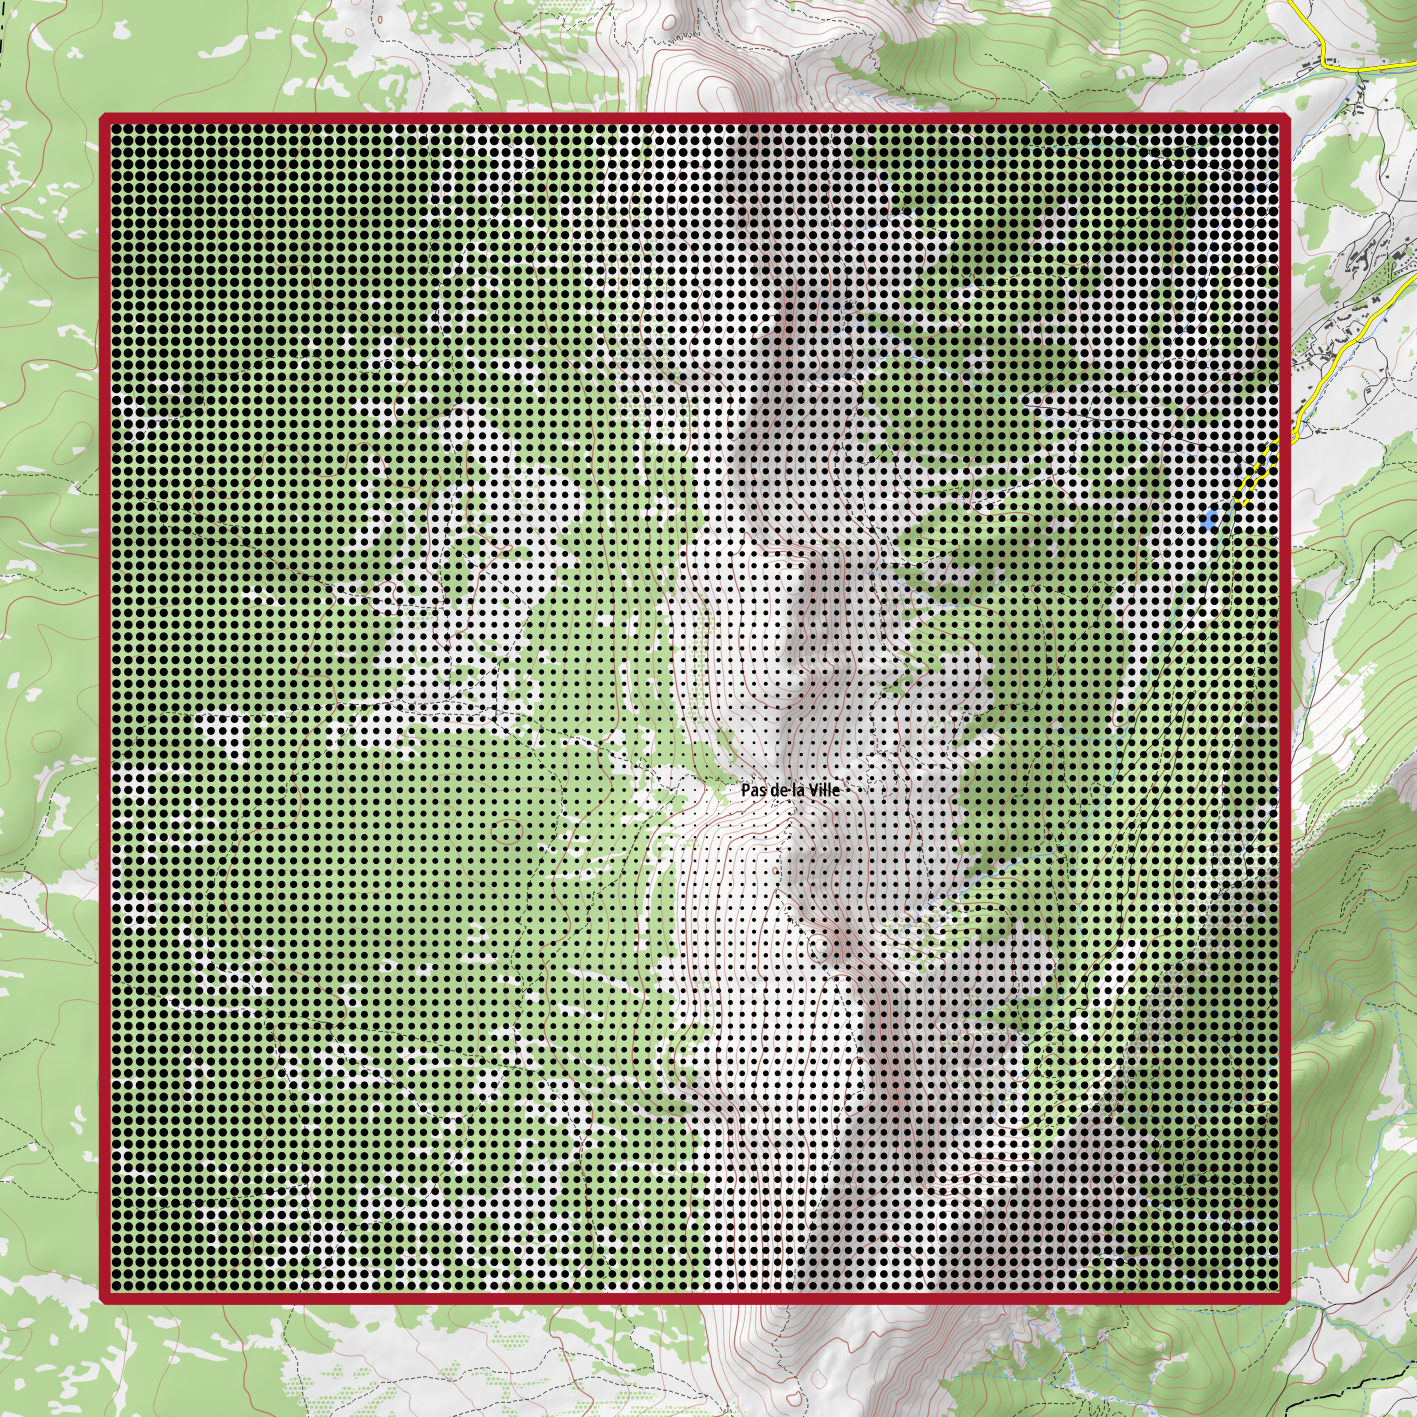
\includegraphics{./figures/Distance_PasVille.png}};
  % 
  \begin{scope}
    \node (P2) at ([yshift=-.5cm]image.south east) {};
    \node (P1) at ([yshift=-.5cm]image.south west) {};
    % 
    \node (rect) [anchor=north west, minimum width=1cm,minimum
    height=.25cm] at ([yshift=-.25cm]P1) {}; \path[draw=RdBu-9-1, line
    width=1mm](rect.west) --([xshift=-1ex]rect.south) -- ([xshift=1ex]rect.north)
    -- (rect.east);
    % 
    \node[anchor=west, font=\tiny\vphantom{Ag}, text width = 4cm] at
    ([xshift=1ex]rect.east) {Limite de la \ac{zir}};
    %
    \node[anchor=west, font=\footnotesize\vphantom{Ag}] at
    (P1 |- 0cm,-1.7cm) {Distance au \emph{Pas de la Ville :}};
    %
    \begin{scope}
      \foreach \x [evaluate=\xshift using 1+\x/10, evaluate=\rad using (\x * .0004) + .01] in {0,...,100}
      {
        \draw[fill=black,draw=none, below] ([xshift=\xshift cm, yshift=-2cm]P1) circle [radius=\rad cm];
      }
      % 
      \path(1,-2.5) --++ (10,0)
      node[et,pos=0] {\SI{0}{\meter}}
      node[et,pos=.5] {\SI{2500}{\meter}}
      node[et,pos=1] {\SI{5000}{\meter}};
    \end{scope}

    % Échelle
    \draw[-] (P2 |- -1cm,-1cm) --++ (-1,0) node[et,pos=.5] {\SI{500}{\meter}};
    % Légende détaillée
    \path (P1) -- (P2) node[pos=.5, yshift=-2.5cm] {\tiny Pour la légende détaillée du fond topographique voir \autoref{anx:topo_leg}. Sources: BD TOPO 2018, BD ALTI 2018.}; 
  \end{scope}
\end{tikzpicture}
  \caption{Métrique \protect\onto[orla]{Distance}, calculée pour la
    spatialisation de la relation de localisation atomique
    \protect\onto[orla]{Distance\-Pla\-ni\-mé\-trique}.}
  \label{fig:veyont_distance}
\end{figure}

Pour construire la \ac{zlc} spatialisant cet indice de localisation il
est ensuite nécessaire de \emph{fuzzyfier} la métrique
(\autoref{fig:veyont_distance}) à l'aide du fuzzyficateur
\onto[orla]{Eq\-Val}.

\begin{figure}
  \centering
  \begin{tikzpicture}[scale=.7]
  \def\decalageX{-.2}
  \def\decalageY{-.2}
  % Courbe
  \begin{scope}[transparency group]
    % fond
    \begin{scope}
      \path[ffa]  (3,0) -- (4.5, 2) -- (6,0) -- cycle;
    \end{scope}
    % bords
    \begin{scope}
      \path[ffc] (1,.8) -- (3.6,.8) -- (4.5, 2) -- (5.4,.8) -- (8,.8) ;
      \path[ffc_fade_m] (0,.8) -- (1,.8) ;
      \path[ffc_fade] (8,.8) -- (9,.8) ;
    \end{scope}
  \end{scope}
  % Axes X, Y
  \begin{scope}
    % Axe X
    \begin{scope}
      % Axe
      \draw[<->] (0, \decalageX) --++ (9, 0) coordinate (x axis);
      % Graduations
      \foreach \n/\t in {0.5/{},1.5/{},2.5/{400},3.5/{},4.5/{800},5.5/{},6.5/{1200},7.5/{},8.5/{}}
      {
        \draw[-] (\n, \decalageX - .05) --++ (0, .1);
        \node[below, font=\footnotesize] at (\n, \decalageX - .05) {\t};
      }
      % label
      \node[below left, yshift=-.1cm, font=\small] at (x axis)
      {\itshape Distance \normalfont (m)};
    \end{scope}
    % Axe Y
    \begin{scope}
      % Axe
      \draw[-] (\decalageY ,0) --++ (0, 2) coordinate (y axis);
      % Graduations
      \foreach \n/\t in {0/{0},2/{1}}
      {
        \draw[-] (\decalageY -.05, \n) --++ (.1, 0);
        \node[left, font=\footnotesize] at (\decalageY -.05, \n) {\t};
      }
      % Label
      \node[above] at (y axis) {$\mu$};
    \end{scope}
  \end{scope}
  \begin{scope}
    % Seuil 1
    \draw[ffc,line width=.5] (3,\decalageY) -- (3,0);
    \draw[fill, RdBu-9-1] (3,\decalageY) circle (2pt);
    \draw[fill, RdBu-9-1] (3,0) circle (2pt);
    % Seuil 2
    \draw[ffc,line width=.5] (4.5,\decalageY) -- (4.5,2);
    \draw[fill, RdBu-9-1] (4.5,\decalageY) circle (2pt);
    \draw[fill, RdBu-9-1] (4.5,2) circle (2pt);
    % Seuil 3
    \draw[ffc,line width=.5] (6,\decalageY) -- (6,0);
    \draw[fill, RdBu-9-1] (6,\decalageY) circle (2pt);
    \draw[fill, RdBu-9-1] (6,0) circle (2pt);
  \end{scope}
\end{tikzpicture}

  \caption{XXXX \enquote{Grand Veymont}}
  \label{fig:fuzzy_veyont_distance}
\end{figure}







\subsubsection{Construction de la zone de localisation probable}

À la suite de la spatialisation des différents indices de localisation
et de la composition des 

\subsection{Critique de la modélisation}
\label{subsec:9-2-3}

\tdi{Impact de la position du toponyme "pas de la ville" sur la
  modélisation}

Un autre problème notable est l'impact que peut avoir la géométrie des
objets de référence sur le résultat de la spatialisation. Par exemple,
l'indice de localisation : \enquote{À \SI{800}{\meter} du Pas de la
  Ville} a été spatialisé en calculant la métrique
\onto[orla]{Distance} à partir du ponctuel plaçant l'oronyme
\enquote{Pas de la Ville} dans la base de données. Or, la
représentation d'un géotype étendu, comme un pas ou une crête, par un
point est une approximation conséquente, impactant fortement la
spatialisation.


%%% Local Variables:
%%% mode: latex
%%% TeX-master: "../../../../main"
%%% End:
